\section{Computational Analysis}
\label{sec:motivaiton}

We analyze how MoE-based LLMs with MHA or GQA perform on a multi-GPU system and explore available options to enhance the performance.
We follow the data/model/expert parallelism methodologies from \cite{icml-2022-DSMoE} for the job distribution among the GPUs.
Fig.~\ref{fig:gpu_distribution} shows an exemplar model distribution of an LLM with four expert FFNs in the system consisting of two nodes with two GPUs each.
The system uses expert parallelism for the MoE layers, which distributes expert FFNs across the GPUs.\footnote{If the number of GPUs ($N_{\text{GPUs}}$) exceeds the number of experts, then each expert is allocated \(\frac{N_{\text{GPUs}}}{N_{\text{ex}}}\) GPUs using tensor parallelism.}
For the FC layers excluding MoE, the system uses tensor parallelism by partitioning rows or columns of a weight matrix within a node and data parallelism by distributing requests across the nodes.


\subsection{Computational Analysis of MoE and Attention Layers}
\label{sec:motivation:compute_analysis}

The MoE and attention layers are dominant in both the \deconlystage and the \mixedstage (Fig.~\ref{fig:roofline}(a)).
Although adopting MoE increases the amount of computation just by $k$, the number of expert FFNs chosen by a gate (\eg, $k=2$~\cite{icml-2022-GLaM, arxiv-2024-mixtral, grok1}), independent requests as a whole are expected to explore most of the expert FFNs in the model (\Numex);
thus, memory access skyrockets to load \Numex expert FFNs, which in turn raises latency.
In the case of the attention layer, as shown in prior work~\cite{asplos-2024-attacc}, the throughput improvement from batching diminishes because each request accompanies its own KV matrices.
Therefore, as the sequence length and the batch size increase, the significance of attention layers increases.

MoE and attention layers exhibit low \opb in the \deconlystage (see Fig.~\ref{fig:roofline}(b)), which severely reduces GPU utilization.
Compute utilization becomes lower than 11\% for the MoE layer and 2.06\% for the attention layer on GPUs.
Because the tokens in the batch are distributed among the experts by gate, each expert processes a relatively small number of tokens because $k$ is smaller than \Numex.
Still, multiple requests can share the same expert, resulting in the \opb becoming higher than one.
Second, as multiple heads share KV matrices, the attention layer exhibits higher \opb for GQA (Mixtral) than for MHA (GLaM), but \opb remains low even with GQA.
Unique KV matrices exist for each request and for each head (MHA) or each group (GQA), resulting in a GEMV with a Q vector or a GEMM with a narrow \deggrp-wide Q matrix, where \deggrp ranges from four to eight~\cite{arxiv-2024-mixtral, grok1, arxiv-2023-llama2}.
This computation exhibits low \opb.


\begin{figure*}[!tb]
  \center
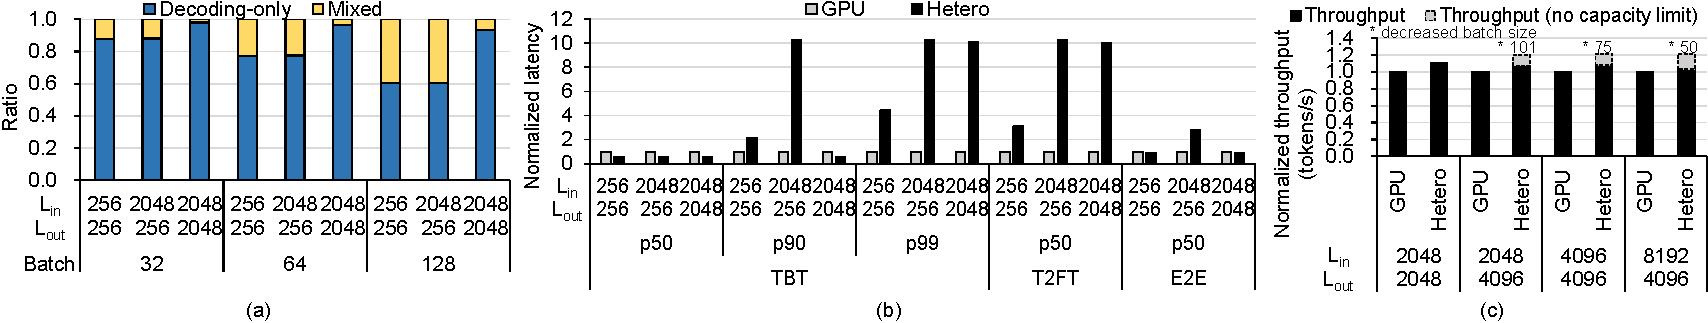
\includegraphics[width=0.99\textwidth]{figures/motivation_latency_bar_rev.pdf}
  \vspace{-0.1in}
  \caption{(a) The ratio of \deconlystage to \mixedstage in \mixtral on a GPU system. (b) The normalized latency of a heterogeneous system compared to a \gpu system in \mixtral with a batch size of 32. The \gpu system consists of four GPUs, while the heterogeneous system consists of two GPUs and two \lowp{s} (details in Section~\ref{sec:duplex}). (c) The normalized throughput of the heterogeneous system over the \gpu system in \mixtral with a batch size of 128.
  }
  \label{fig:latency_cdf}
  \vspace{-0.1in}
\end{figure*}

The request batch size also significantly impacts the \opb except for the attention layer, which is performed separately for each request.
In particular, utilizing a larger batch size increases the \opb of the MoE layer as more requests in a batch share the same expert.
Nevertheless, for practical batch sizes abiding by the latency limitation imposed by the service level objective (SLO) and memory capacity for KV matrices, the attention and MoE layers stay in the low \opb region.

In the case of \mixedstage, the \opb of MoE and attention layers increases.
A new request added to \mixedstage increases the number of tokens that select each expert, increasing the \opb of the MoE layer.
The new request causes numerous tokens, much more than \deconlystage by $L_{in}$, pass through the MoE layer, resulting in a higher number of tokens processed per expert.
In the attention layer, the operation for the new request exhibits a high \opb because $L_{in}$ Q slices share the same KV matrices for each head.


\subsection{Limitations of Heterogeneous Systems}
\label{sec:motivation:hetero_limitations}
We discover that most stages in LLM inference with continuous batching are \deconlystage{s}.
This is because each request consists of a single prefill stage and multiple ($L_{out}$) decoding stages.
Fig.~\ref{fig:latency_cdf}(a) shows the ratio of decode-only and mixed stages in Mixtral for various $L_{in}$ and $L_{out}$ values in a four-GPU system (detailed in Section~\ref{sec:experimental_setup}).
It can be observed that the \deconlystage is dominant for all cases.
Thus, it is important to quickly process the \deconlystage to reduce the \ete latency and improve serving throughput.

To accelerate the \deconlystage, it is necessary to speed up the MoE layers and attention operations, which occupy most of the time in the \deconlystage and have low-\opb characteristics. Hence, one can design a heterogeneous system (hetero system)~\cite{asplos-2024-attacc} that includes device nodes with high memory bandwidth and low computing power dedicated to MoE and attention layers alongside conventional GPUs.
We suppose such a hetero system consisting of two GPUs and two \lowp(detailed in Section~\ref{sec:duplex}) and compare it with a four-GPU system.
We assume that the \lowp processes all MoE layers of all stages and the attention operations of \deconlystage{s} to avoid MoE weight duplication.
This hetero system can reduce the median (p50) \tbt and \ete latency as shown in Fig.~\ref{fig:latency_cdf}(b).

However, the 90th (p90) and 99th (p99) percentile \tbt and median \ttft latency values show significant increases due to the limited computing power of the devices targeting low-\opb operations.
As the MoE layers exhibit high 
\opb in the \mixedstage, devices with high memory bandwidth but low computing power become severely compute-bound for these layers. 
As \lin increases, the higher \opb in the MoE layer leads to increased \ttft and tail latency in \tbt, and even in \ete for some cases. 
\tbt and \ttft are critical performance metrics for LLM inference, especially in conversational tasks~\cite{isca-2024-splitwise}, which often involve multiple rounds of dialogues between the user and the chatbot.
Because each round is processed as a separate request, \lin continues to increase as the conversation progresses, exacerbating the problem.

To prevent the tail latency from skyrocketing, it is necessary to duplicate the weights of the MoE layers on GPUs with high computing power and process the MoE layer of the \mixedstage on these GPUs.
However, duplicating the weight of MoE layers, which take the most model weights, is highly inefficient, requiring more devices due to limited memory capacity.
Further, such hetero systems limit memory capacity for KV matrices, which increases proportionally to batch size, than homogeneous systems, thereby reducing the maximum batch size and thus hindering system throughput (see Fig.~\ref{fig:latency_cdf}(c)).

